\documentclass[11pt]{article}
\usepackage{graphicx}
\usepackage{listings}
\sloppy
\begin{document}
\title{PROCESSOR DESIGN AND DATAPATH DESIGN IN VERILOG}
\author{Anurag Pallaprolu\\2012B5A3405P\\SK 207, BITS Pilani}
\maketitle
\tableofcontents
\setcounter{tocdepth}{3}
\section{Introduction}
This document deals with the different types of processor designs and how the respective datapaths can be simulated in Verilog. It is clasiified into components needed to build a datapath for a relatively simple MIPS instruction. Each component will be described and a sample Verilog implementation is displayed. It might not be the most efficient design but the implementation is assured to work. Then, I would look at designing processors in three basic types of design.
\begin{description}
	\item[Single Cycle] \hfill \\
	This design basically tries running the entire instruction in one cycle always. This is the chronologically first type of processors that were made. It is inefficient for the obvious reason that, for the entire instruction to run in one cycle, the cycle length should be larger than the slowest instruction. Hence, the computation efficiency will also go by the same proportion.
	\item[Multi Cycle] \hfill \\
	As the name suggests, multicycle or multiple cycle implementation essentially implements each of the sub-implementations in their respective cycles. It still appears as if this still has the "cycle time greater than the time of slowest instruction" problem but care must be taken as the instruction that we are talking about here is the subimplementation of the actual instruction. So, it is not an actual disadvantage but the cycle time is assured to be shorter than the single cycle design.
	\item[Pipelined] \hfill \\
	This is a radical shift from the above two types. It essentially implements an assembly line type of processing the sub-implementations of the given instruction. But, this time, the cycle length depends on the number of so called "pipelines". I shall explain more about the associated terminology later. But I suppose the picture below should suffice.

\end{description}

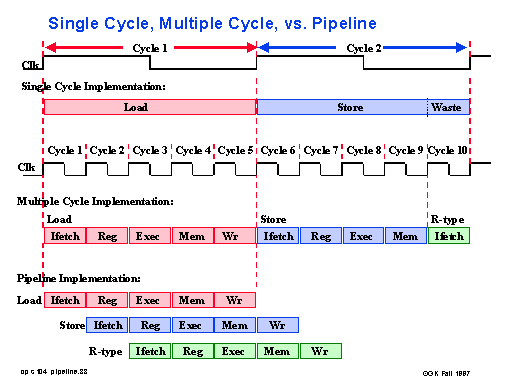
\includegraphics[scale=1.15]{smpp.png}
In the upcoming sections, I would review my basic digital devices to build a datapath in verilog. But first, something traditional related to Verilog.
\section{The Language: Testbenches}
Any Verilog code written will have to be tested on a given number of input values. The place where you (virtually) go out to test your device is called the Testbench. In this case, it is a Verilog file with a module assigned to it. As an example, take a look at the Verilog code for a D Flip Flop and the Testbench for the corresponding device. The details of the specific device will be dealt with later.
\begin{description}
	\item[The Module] \hfill \\
	\lstinputlisting[language=Verilog]{dff.v}
	\item[The Testbench] \hfill \\
	\lstinputlisting[language=Verilog]{dff_tb.v}
\end{description}

So it is quite clear to see what a Testbench does. It sets up a loop of values which are ran on the given device and its output is recorded. Note: The commands $dumpfile()$ and $dumpvars()$ are NOT related to Verilog. They are parameters for viewing the wave diagrams and are needed for waveform viewers like GTKWave etc. If you are using a standard verilog compiler like $iVerilog$ then the dump file can be created easily by the following command $> iverilog -o *enter exec name* *enter tb name* *enter src name*.$
\section{The Components}
\subsection{Multiplexor}
The multiplexor or more commonly known as a "mux" is a basic digital circuit which essentially lets the user choose one input from the given array of several inputs. This is implemented quite easily in a behavioral manner in Verilog, but the circuit is also quite simple. The multiplexor is a very versatile device when it comes to decision making situations in circuits quite easy to implement. The schematic is given below and then the Verilog code(s) to implement this design.

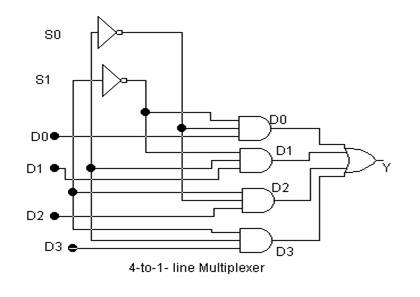
\includegraphics[scale=1.15]{image010.jpg}

The essential idea is to take in the values of the select lines and allow the corresponding data lines through. The behavioral Verilog code is given below.
\lstinputlisting[language=Verilog]{mux.v}
The Verilog code for the gate level design schematic shown before is given below.
\lstinputlisting[language=Verilog]{mux2.v}

\subsection{Adders and Subtractors: The basic Arithmetic Logic Unit}
An Arithmetic Logic Unit(ALU) has the basic function of performing arithmetic on given input bits. The type of operations to be done are specified by the appropriate control lines. The most basic of arithmetic operations that can be done are addition and subtraction. Devices which perform such tasks are called "adders". Another control line to the adder(called the "binvert")can be summoned to make it sign-invert one of the bits and then add them, a process equivalent to subtraction.

There are essentially two types of adders. Ones which cannot accomodate for overflow(sometimes also known as carry out/carry in) are called as half-adders. Adders which have three input pins and two output pins two extra for the two overflow pins are called full adders.

The design for a half adder is given below.




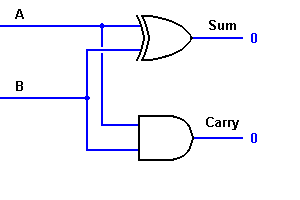
\includegraphics[scale=1.15]{Half-Adder-Circuit.png}
\lstinputlisting[language=Verilog]{ha.v}
The design for the full adder is given in the next page. Notice the slight similarity in the first stage of arrangement.

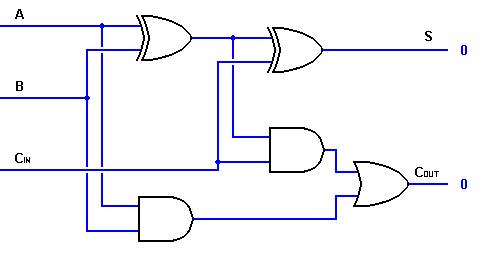
\includegraphics[scale=1]{Full-Adder-Circuit.png}

\lstinputlisting[language=Verilog]{fa.v}

Making a subtractor need not be dealt in detail because the only change in both the circuits is just at inverting a signal(if its a one bit scenario then by a not gate). I can now extend the number of input bits required by the adder. The schematic for the "ripple-carry adder" is given below.
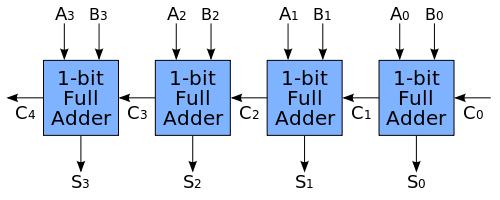
\includegraphics[scale=0.75]{rca.png}

\subsection{Latches, Flip Flops and Registers: Sequential Digital Devices}
In the entirety of the digital devices that we will see, we can divide them into two categories: Combinational and Sequential Devices. The diagram given below should make things clear regarding the differences between combinational and sequential circuits. 

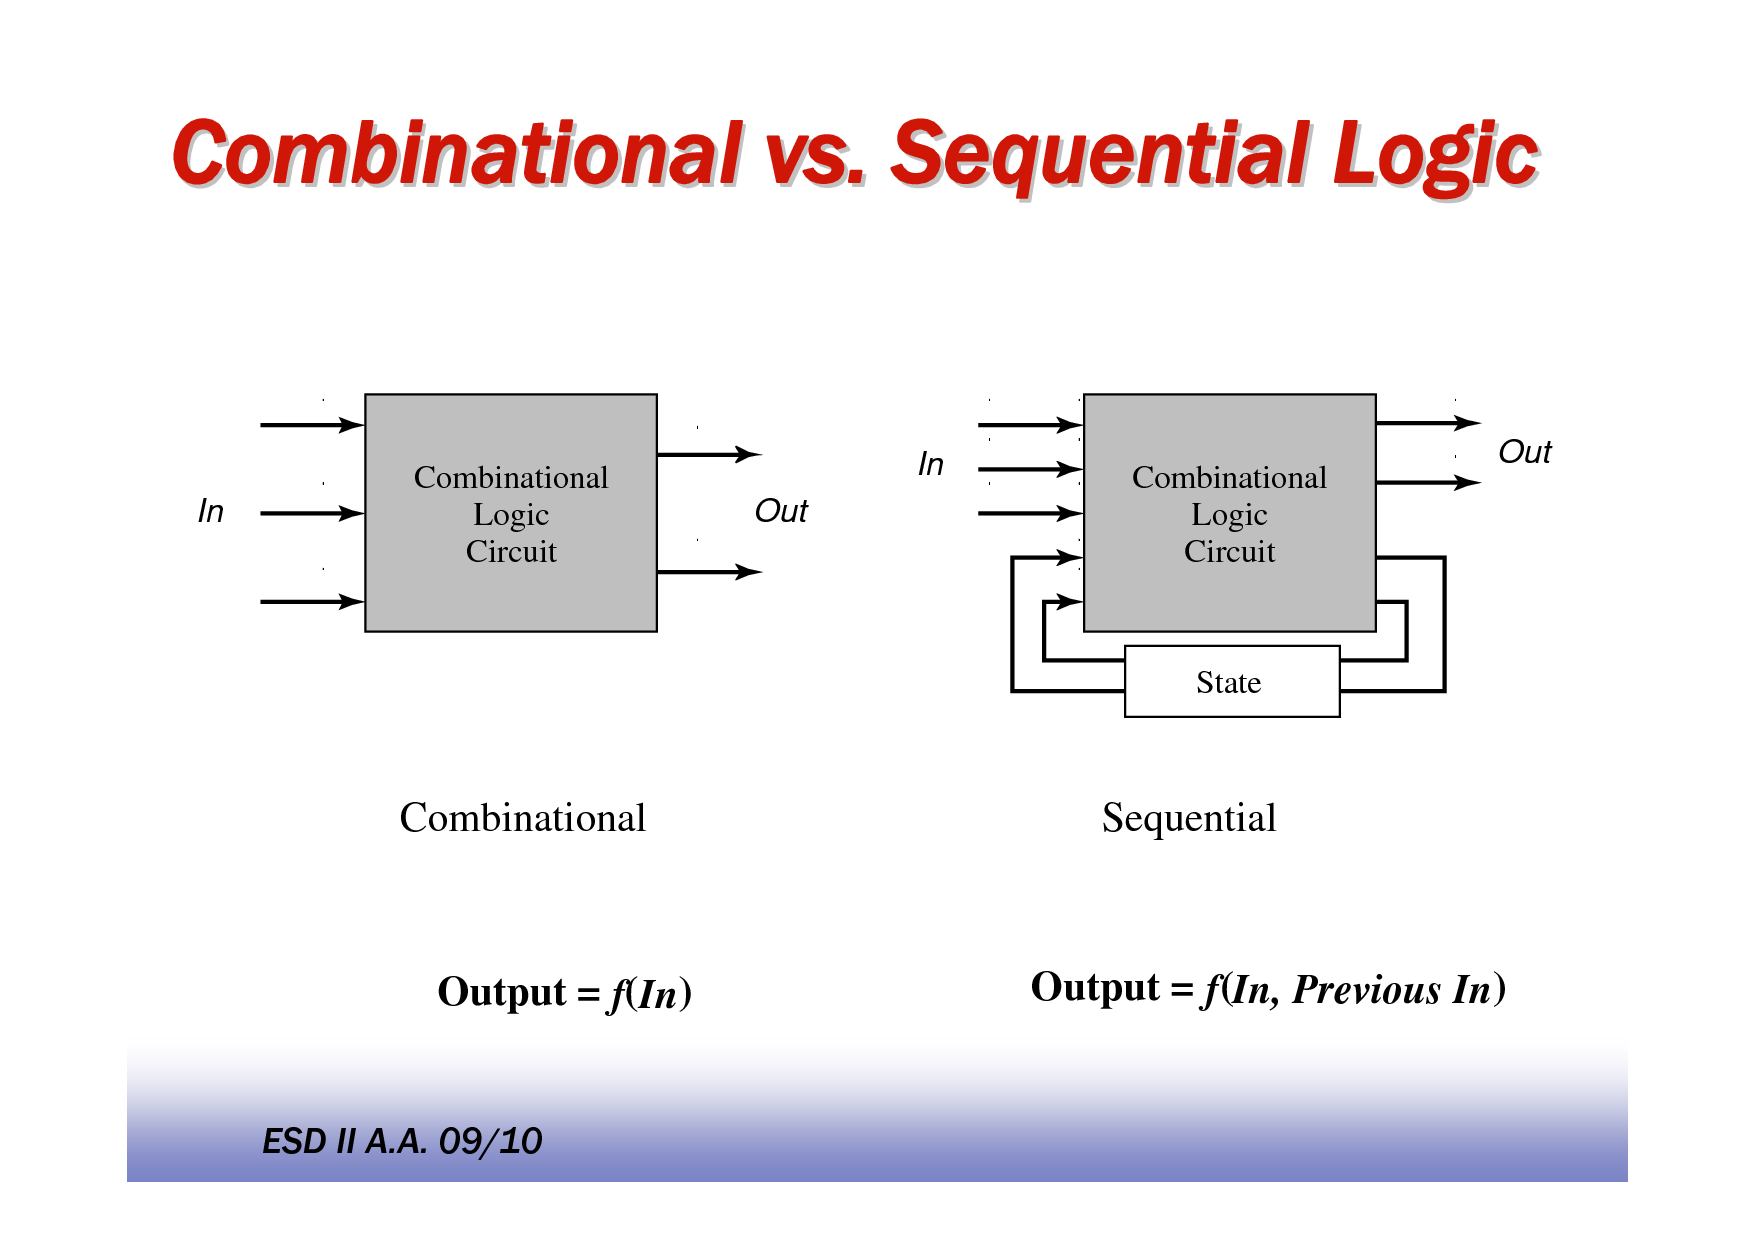
\includegraphics[scale=0.50]{cscir.png}
To repeat, combinational circuits do not involve any sort of storage or memory of sorts, given a live data it works with it on the spot and shoots out the result. A sequential circuit involves some sort of a memory of the given data, the output depends recursively on previous inputs. A combinational logic is neccesary for a sequential circuit to exist. Refer to the figure in the next page.

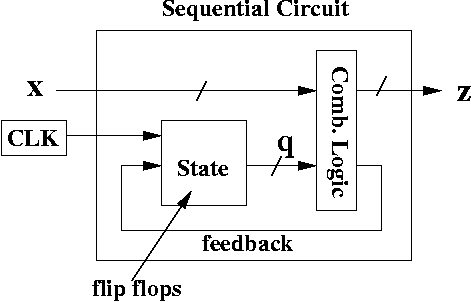
\includegraphics[scale=0.50]{seq.png}


Let us start our memory design section with the simplest of all devices, the latch.
\subsubsection{Latch}
As the name suggests a latch is a single bit storage device which has two states. In more technical language, it is said to be a bistable multivibrator, which means, it has only two stable existant states. Latches can be memory devices, and can store one bit of data for as long as the device is on. As the name suggests, latches are used to "latch onto" information and hold in place. Latches are very similar to flip-flops, but are not synchronous devices, and do not have a visible clocking methodology. There are two basic types of latches manufactured.
\begin{description}
	\item[SR Latch: The Set/Reset Latch] \hfill \\
	An SR Latch is an asynchronous i.e, non clocked device. It works independently of control signals and relies only on the state of the S and R inputs. The schematics for the SR Latch are given below. Starting from the block diagram to the gate level implementation are presented.

	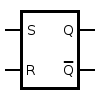
\includegraphics[scale=1]{srl1.png}
	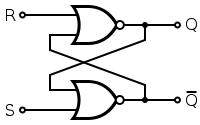
\includegraphics[scale=1]{srl2.png}
	\item[Gated SR Latch] \hfill \\
	In simple words, the Gated SR latch is a slight improvement, more rather a modification in which the latch's working condition i.e, its control could be enabled or disabled as per usage. There is an extra input port for enabling and disabling the latch. The schematic is given below.
	
	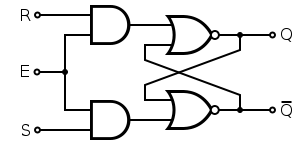
\includegraphics[scale=1]{gsrl.png}
	\item[D Latch] \hfill \\
	The D-Latch is an abbreviation of Data Latch. It is a more data secured kind of a gated SR Latch. There are two input pins, one for data and other for enabling the latch. There are no more set and reset pins. The schematic is as follows:

	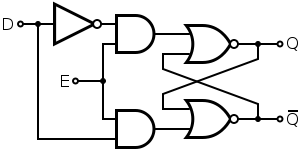
\includegraphics[scale=1]{dl.png}
\end{description}

The Verilog code for the corresponding types of latches is given below. 
\begin{description}
	\item[D Latch] \hfill \\
	\lstinputlisting[language=Verilog]{dl.v}
	\item[Gated S-R Latch] \hfill \\
	\lstinputlisting[language=Verilog]{gsr.v}
\end{description}

\subsubsection{Flip Flops}
Flip flops are traditional to memory devices. They can be thought of simply as one bit registers. In the very essence, a flip flop is similar to a latch, with the only stark difference being the fact that Flip Flops have a kind of a feedback mechanism which helps them hold onto the assigned value. Changes in data stored will be visible only at positive edges of clocks. I have mentioned before a type of a flip flop(the DFF) at the beginning while talking about testbenches. I would explain two more types of flip flops. First the schematics and then the Verilog.
\begin{description}
	\item[SR Flip Flop] \hfill \\
	An SR(Set/Reset) flip-flop is perhaps the simplest flip-flop, and is very similar to the SR latch, other than for the fact that it only transitions on clock edges.	SR flip-flops are extremely uncommon because they retain the illegal state when both S and R are asserted. Generally when people refer to SR flip-flops, they mean SR latches. The Verilog code is easy to understand.
	\lstinputlisting[language=Verilog]{sff.v}
	\item[D Flip Flop] \hfill \\
	A D Flip Flop is the most common kind of flip flop which is used mostly to make registers and register files. They are the edge triggered variant of the transparent latch. It has a standard symbol given below.
	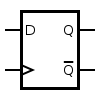
\includegraphics[scale=1]{dff.png}
	The Verilog code for the DFF has been given in section 2 itself. Refer it for the testbench too. 
	\item[JK Flip Flop] \hfill \\
	The JK flip flop is just an advanced SR type flip flop. The only improvement is in terms of the stability. Note the fact that, when both the inputs of the SR flip flop are 1, then the device goes into a metastable state, whereas in a JK flip flop it does the job of inverting the signal. Refer to the table given below for clarity. The first table is about SR flip flops
\begin{center}
	\begin{tabular}{ | l | l | l | l | p{5cm}  |}
	\hline
	S&R&Q&Comment \\ \hline
	0&0&0&Hold State \\ \hline
	0&1&0&Reset \\ \hline
	1&0&1&Set \\ \hline
	1&1&Meta&stable \\ \hline
	\hline
	\end{tabular}
\end{center}
	The table below is for JK flip flops. Q* refers to the complement of Q.
\begin{center}
	\begin{tabular}{ | l | l | l | l | p{5cm}  |}
	\hline
	J&K&Q&Comment \\ \hline
	0&0&Q(previous)&Hold \\ \hline
	0&1&0&Reset \\ \hline
	1&1&$Q*$&Toggle \\ \hline
	\hline
	\end{tabular}
\end{center}

\subsubsection{Registers}
I had mentioned before that D flip flops can be used to create register memories. Now, we shall actually build a 32 bit register using 32 individual flip flops. You might think that synchronization of those many bits of data would be difficult, but it is all managed thanks to the simultaneous clock line that runs through all of them. The schematic and the Verilog implementation are given below.

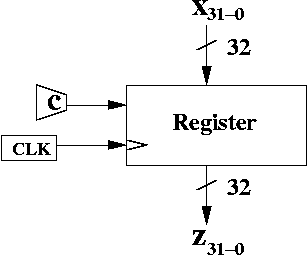
\includegraphics[scale=0.7]{pload.png}

\lstinputlisting[language=Verilog]{reg32b.v}

Here, again, the language comes to the aid. The command $genvar$ sets up a running variable which then generates parallel instances of the same device. $generate$ and $endgenerate$ mark out the replication part of the code.
\subsubsection{Register Files}
Now, I move up the strucure of data storage sizes and we can see clearly that the next obvious choice of such devices is to collect many 32 bit registers into a sort of a "mega-register". This is nothing but a plain old register file. A simple diagram is given next page which explains the concept. 

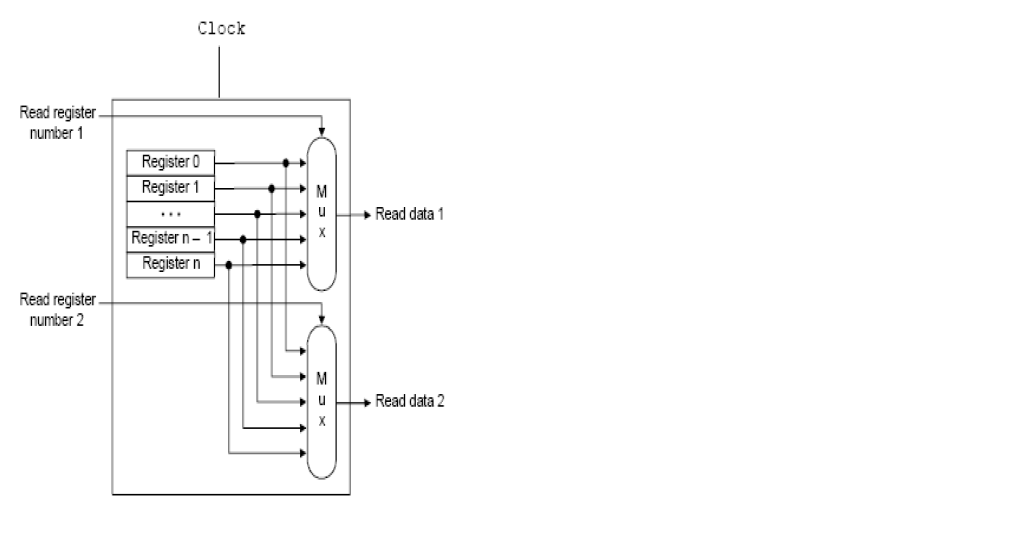
\includegraphics[scale=0.7]{regfile.png}

The register files are stacked up and each one can be summoned by calling their appropriate 5 bit register number. The multiplexors help us in selecting the right register number and supplying us with the data in the register. It is no surprise that the writing of data into the registers is very similar to the reading procedure and this will be discussed in the next few pages. Now, for the larger picture, the Verilog code.



\lstinputlisting[language=Verilog]{regfile.v}

I have not written the $regfile$ module altogether because the above script contains all the subcomponents of the file. All that is left to implement is keeping track of registers and implementing the correct select lines. The block diagram schematic makes this point clear
The write procedure for a register file, does however involve some differences, like the write synchronization with the clocking etc,. The block diagram for the writing method is given below. It involves the same stack to be rewritten into the data from the given register number.
 
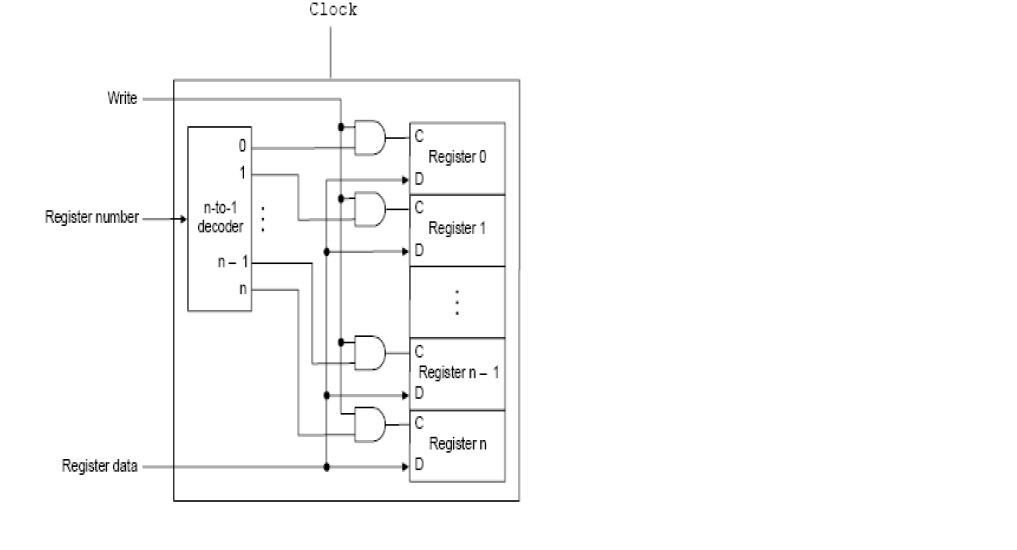
\includegraphics[scale=0.7]{write.png}

Note: The component n to 1 decoder or simply a $decoder$ is a digital device which has the task of setting one of the outputs in the given array of outputs as high and the remaining low. Technical jargon aside, it is very similar to the operation of a multiplexor.  For a much simpler understanding, look at the schematic and the truth table followed by it.

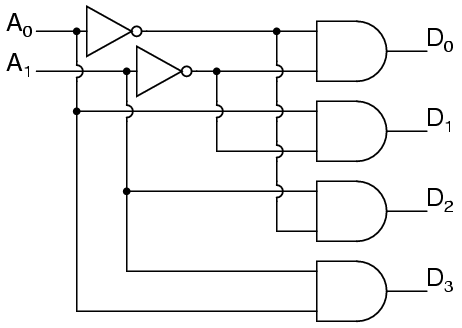
\includegraphics[scale=0.7]{dec.png}

\begin{center}
	\begin{tabular}{ | l | l | l | l | l | l |}
	\hline
	A1&A0&D3&D2&D1&D0 \\ \hline
	0&0&0&0&0&1 \\ \hline
	0&1&0&0&1&0 \\ \hline
	1&0&0&1&0&0 \\ \hline
	1&1&1&0&0&0 \\ \hline
	\hline
	\end{tabular}
\end{center}

A simple script for the gate level design of the decoder is given below.
\lstinputlisting[language=Verilog]{dec.v}

I have $almost$ come to an end to the description of the toolchain we would use to build a basic datapath. $However$, I would now describe the fully functional Arithmetic Logic Unit.

\subsection{Arithmetic Logic Unit: A mix of things}
As explained in a previous section, the ALU is the mothership for all arithmetic operations on data incoming from a register file. The methods in which data flows along through the ALU will be covered in more detail when I explain what a $datapath$ is. For now, I shall explain the 1 bit ALU. Look at the schematic below.

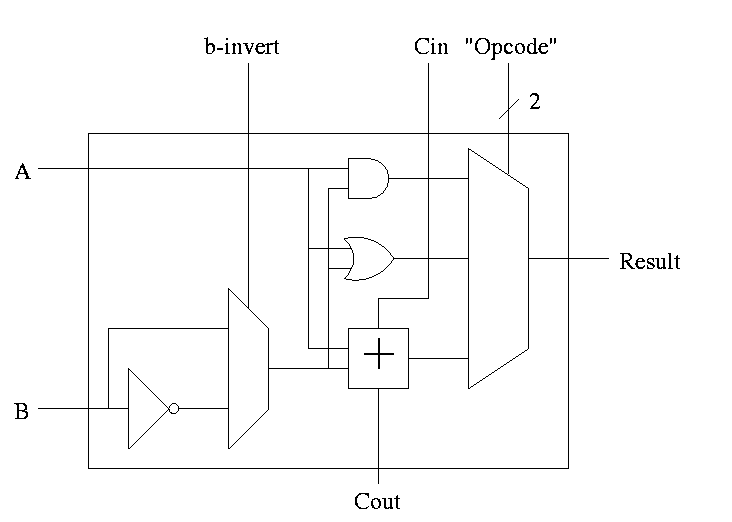
\includegraphics[scale=0.6]{alu1.png}
There are two inputs A and B for logical operations, the b-invert for switching from addition mode to subtraction mode(quite simply by adding the negated value of B), the Cin for any carry-ins entering the full adder inside the ALU. The input $opcode$ (a 2 bit input) is the control line for the mux inside to select the operation the ALU has to perform. The result and cout are the standard output bits as usual.

The $block$ module in the Verilog script on the next page represents the ALU block shown above.

\lstinputlisting[language=Verilog]{alu1.v}

Now we look into the extension of this block unit. Let us see the schematic of a 32 bit ALU below.

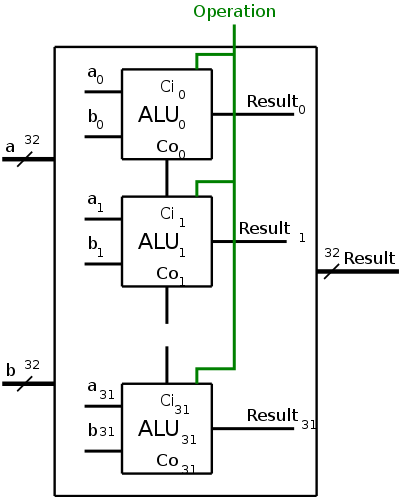
\includegraphics[scale=0.5]{alu-32bit.png}

It is just following the general pattern of clustering digital devices to make a device of larger utility. Programming this is Verilog is also not difficult, noting the use of the generate command and running it through all the, luckily, independent inputs. People generally try to vary the design of the interconnection of the full adders inside the ALU for maximum efficiency. One such design, which we have seen before is the ripple carry adder. There is another eponymous design called the carry lookahead adder whose schematic is shown on the next page.
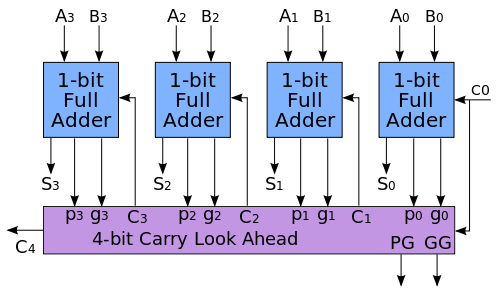
\includegraphics[scale=0.7]{cla.png}

\subsection{Sign Extender/Zero Extender and Logical Left Shifter}
The operation of sign extension is a general term which refers to the process of increasing the number of bits of a binary number while keeping the sign and value preserved. Simply put, it is the process of adding more bits after the most significant bit(MSB). It is used while processing branching instructions for the datapath. The Verilog script for the sign extender is given below. The schematic is not neccesary right now. The symbol for the sign extender is given below.

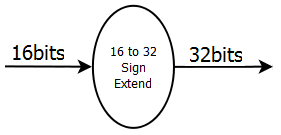
\includegraphics[scale=0.6]{signex.png}




\lstinputlisting[language=Verilog]{Sign_Extend.v}

The Shift Left Logical operation($sll$) is to shift the left most bit in the bit pattern one bit leftwards. This can be clearly seen in the figure below

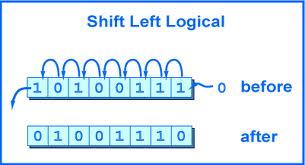
\includegraphics[scale=0.7]{sll.jpg}

The Verilog script:
\lstinputlisting[language=Verilog]{sll.v}

\subsection{A few other useful Verilog scripts}
Now, I am going to show you a few more Verilog scripts which were omitted before due to constraints. I start off with the proper $regfile$ module and include two Verilog scripts from Stanford released open source which contain (maybe) refined versions of my components. 

\subsubsection{RegFile Module}
\lstinputlisting[language=Verilog]{regfile_full.v}

\subsubsection{Stanford Standard Blocks 1}
\lstinputlisting[language=Verilog]{stanford_std1.v}

\subsubsection{Stanford Standard Blocks 2}
\lstinputlisting[language=Verilog]{stanford_std2.v}


\end{description}
\end{document}